\chapter{Implementation - Areas of Application}
\label{ch:impl_aoa}

As described in earlier chapters of this thesis, there are countless applications of graph theory in diverse fields of research and engineering; in order to prove the feasibility of the Graphinius platform, it was necessary to implement a few concrete examples. Consequently, in this chapter we are going to take a look at 3 different Areas of Application that Graphinius (JS, VIS, and eventually the platform) is already able to serve. Amongst these, only the first one can be considered a toy application (although interesting for teaching platforms etc. in itself); graph extraction from images as well as social network anonymization however have been hitherto firmly situated in the realm of servers or entire processing infrastructures.


\section{Manual editing (predefined structures)}
\label{sect:manual_editing}

	The first and foremost use case for Graphinius is simply to be able to interactively build, mutate, and visualize graphs in the browser. Although the final Graphinius Platform will feature a full-blown code editor with code completion and online documentation, the basic functionality can be demonstrated even using a form of REPL every modern browser is automatically equipped with: the debugging console.

	\subsection{Build a graph manually}
	\label{ssect:build_graph_manually}
	
	As depicted in Figure~\ref{fig:build_graph_manually}, the basic case is to create a new graph structure, add some nodes and edges, and then run different computations on it.
	
	\begin{figure}[ht]
		\begin{center}
			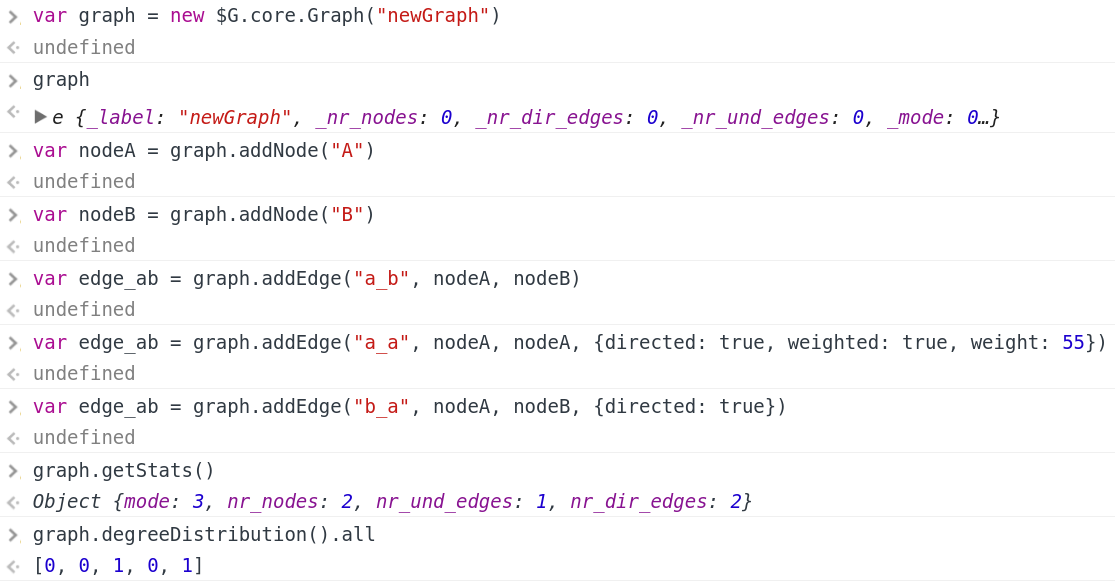
\includegraphics [width=1\textwidth] {figures/buildGraphManually}
			\caption{Manually building a new graph in the console.}
			\label{fig:build_graph_manually}
		\end{center}
	\end{figure}
	
	
	\subsection{Load predefined graph and visualize}
	\label{ssect:load_graph}
	
	Using either the CSV or JSON Reader build into GraphiniusJS, we can also request to instantiate a graph from a remote file. Here we use the JSON Reader to load a graph depicting a nevus and render it using GraphiniusVIS (Figure~\ref{fig:load_graph_repl})
	
	\begin{figure}[H]
		\begin{center}
			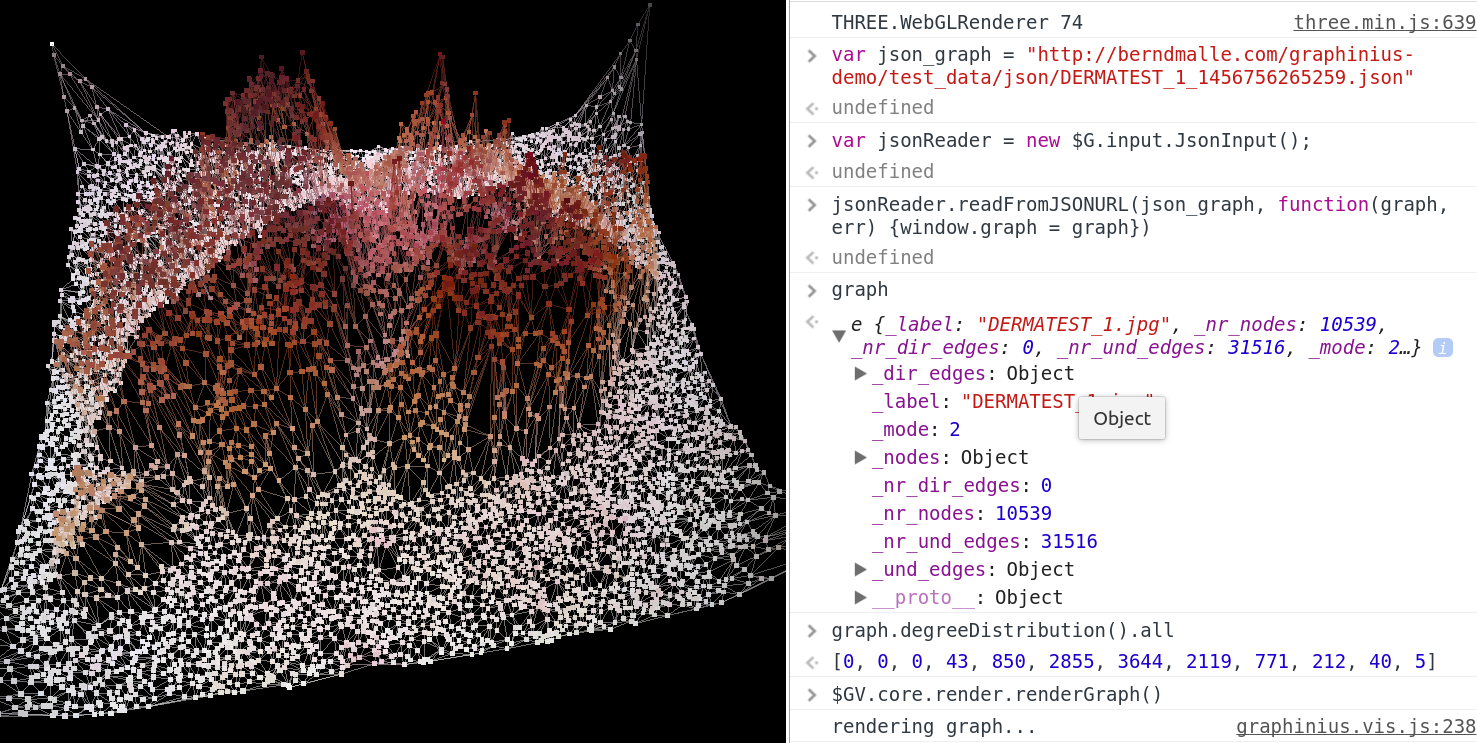
\includegraphics [width=1\textwidth] {figures/loadingGraphInREPL}
			\caption{Loading a JSON graph and visualizing it via the browser console; then determining its degree distribution.}
			\label{fig:load_graph_repl}
		\end{center}
	\end{figure}
	
	
	\subsection{Run a BFS algorithm and visualize}
	\label{ssect:run_bfs_visualize}
	
	After loading a (undirected) graph according to the previous section, we choose a random start node and invoke a breadth-first-search algorithm resulting in a \textit{distance map} centering around that node. The following lines of code (Figure~\ref{fig:color_graph_bfs}) show distances and parents of a selection of nodes (note the parent / distance chain...) while the accompanying visualization colors the graph according to the obtained distances via gradient computations (the start node being colored green and the node with maximum distance being colored red).
	
	\begin{figure}[H]
		\begin{center}
			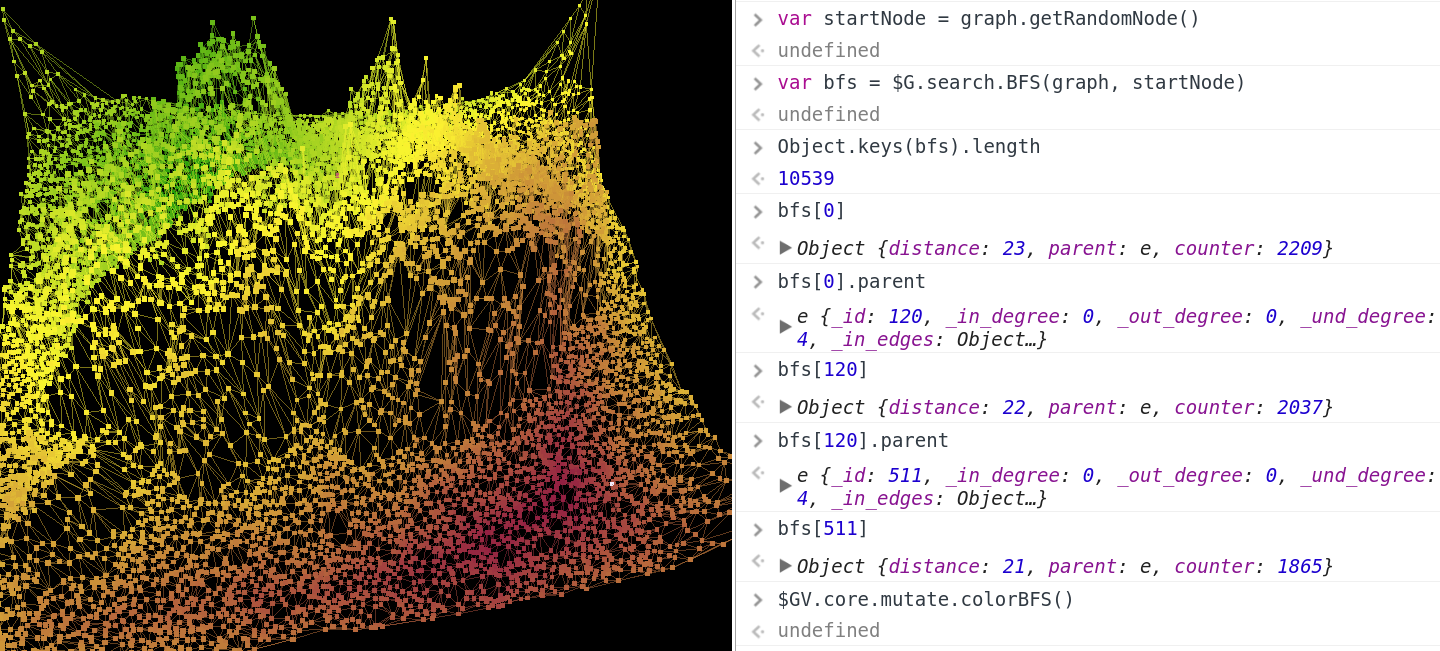
\includegraphics [width=1\textwidth] {figures/colorBFSREPL}
			\caption{Computing a BFS in a live browser REPL \& visualizing the result.}
			\label{fig:color_graph_bfs}
		\end{center}
	\end{figure}
	
	
	\subsection{Run a DFS algorithm and visualize}
	\label{ssect:run_dfs_visualize}
	
	Lastly, in Figure~\ref{fig:color_graph_dfs} we load the same graph as before, this time interpreted as a directed graph, choose a random start node again and invoke a DFS algorithm. This returns to us an array of graph segments representing the node sets reachable from each start node of a respective DFS Visit run (had we chosen an undirected graph, there would only be a single segment). We then output the size of each segment and again visualize the result, assigning to each segment a different color.
	
	\begin{figure}[H]
		\begin{center}
			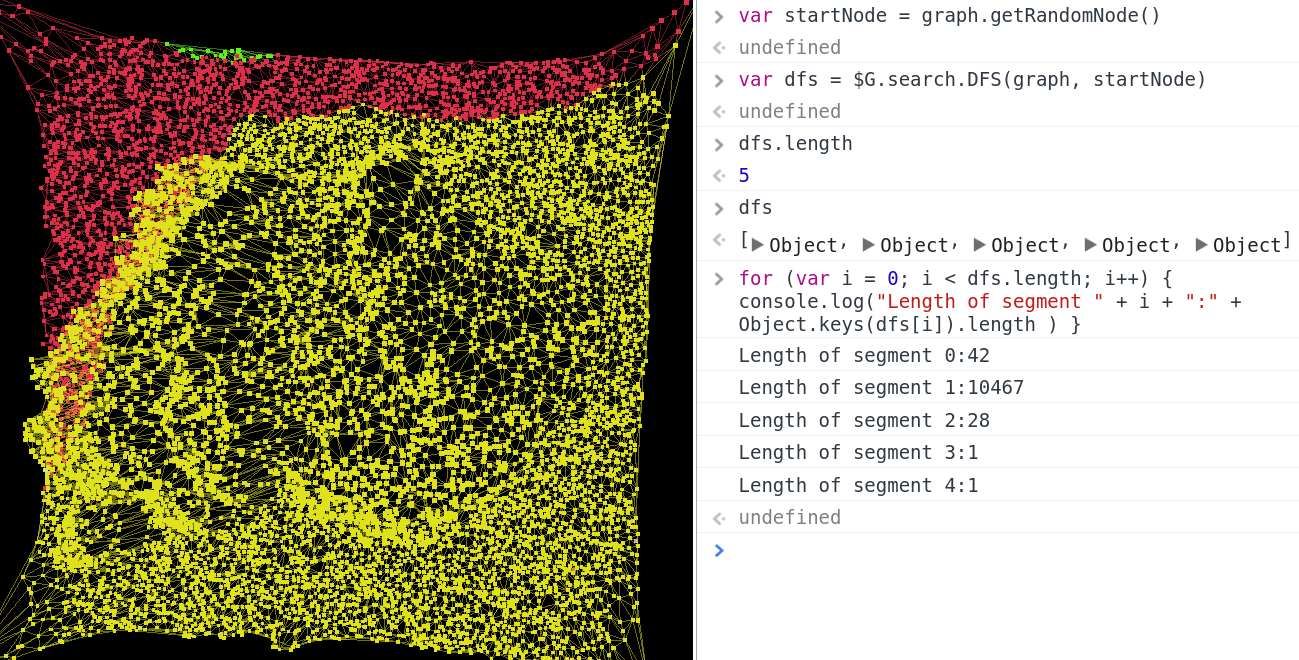
\includegraphics [width=1\textwidth] {figures/colorDFSREPL}
			\caption{Computing a DFS in a live browser REPL \& visualizing the result.}
			\label{fig:color_graph_dfs}
		\end{center}
	\end{figure}	


\section{Graph extraction from images}
\label{sect:graph_ext}
	
	In order to be able to apply graph theory to problems originating in the realm of image processing, first we need to extract a graph structure out of an image. There are potentially many different ways of doing this; as described in our paper \citep{GraphExtractPaper}, we are executing the following steps:
	
	\begin{enumerate}
		\item \textbf{Image preprocessing.} Many image segmentation algorithms use gray scale values to compute distances between neighboring pixels, gradients etc. (it seems that using 3 color channels per pixel is not much superior over using just one).
		\item \textbf{Input image as graph.} The resulting image is simply interpreted as a graph, which is possible because every pixel-based image naturally forms a graph structure, in which pixels are represented by nodes and neighborhoods are represented by edges. We then extract an edge list where the entries is sorted according to edge weight (= differences in the intensity values of neighboring nodes).
		\item \textbf{Graph based (over-)segmentation.} As the next step, a Kruskal MST based algorithm developed by \citep{FelzenszwalbHuttenlocher2004} is applied. It takes the approach of merging regions from pixel level (= inital nodes) 'upwards' instead of recursively partitioning the whole image 'downwards' - essentially, at every step it compares an intra-region coherence measure to an inter-region similarity measure:
		
			\begin{equation*}
			\text{Int}(C) = \max\limits_{e \in \text{MST}(C,E)}  \omega(e)
			\end{equation*}
			is the intra-region coherence value, given by the maximum edge weight of the region's MST.
			
			\par
			\begin{equation*}
			\text{Dif}(C1,C2) = \min\limits_{v_i \in C1, v_j \in C2, (v_i,v_j) \in E} \omega(v_i,v_j)
			\end{equation*}
			denotes the intra-region similarity measure, given by the minimum edge weight connecting any two nodes between them.
			
			\par Finally,
			\begin{equation*}
			\text{D}(C1,C2) = \left\{
			\begin{array}{l l}
			\textit{true} & \quad \text{if} \quad \text{Dif}(C1,C2) > \text{MInt}(C1,C2)\\
			\textit{false} & \quad \text{otherwise}
			\end{array} \right.
			\end{equation*}
			determines if two regions should be merged, based on the relation of their intra-region coherence and inter-region similarity measures.
			
			\par Once all edges have been considered, the final graph partition represents the segmentation (merging) result
		
		\item \textbf{A Delauney triangulation} is computed once the final region map has been established, taking each region's centroid to become a node in the new graph, as well as the (non-overlapping, as the algorithm is producing a tessellation of the region map) connections between those centroids to be their respective edges. The edge weight is computed from the difference in average intensity value of two adjacent regions.

		\item \textbf{Graph output.} Those data are finally transferred into a JSON structure consumable by Graphinius JS, as depicted by the sample JSON graph in Figure~\ref{fig:json_input_graph}.
	\end{enumerate}
	
	With the exception of manually written micro-graphs for the sake of rapid unit testing, this procedure was used for practically all JSON graphs  employed in the development and testing of GraphiniusVIS. Due to the flexibility of the algorithm - it features 3 separate parameters which control the granularity of the partition, and therefore the granularity of the graph structure - it was possible to extract graphs from a few hundred nodes and edges to up to 22k nodes / 66k edges. The average execution time on the author's quad-core i5 machine lay in the range of 3-5 seconds.
		
	\begin{figure}[H]
		\begin{center}
			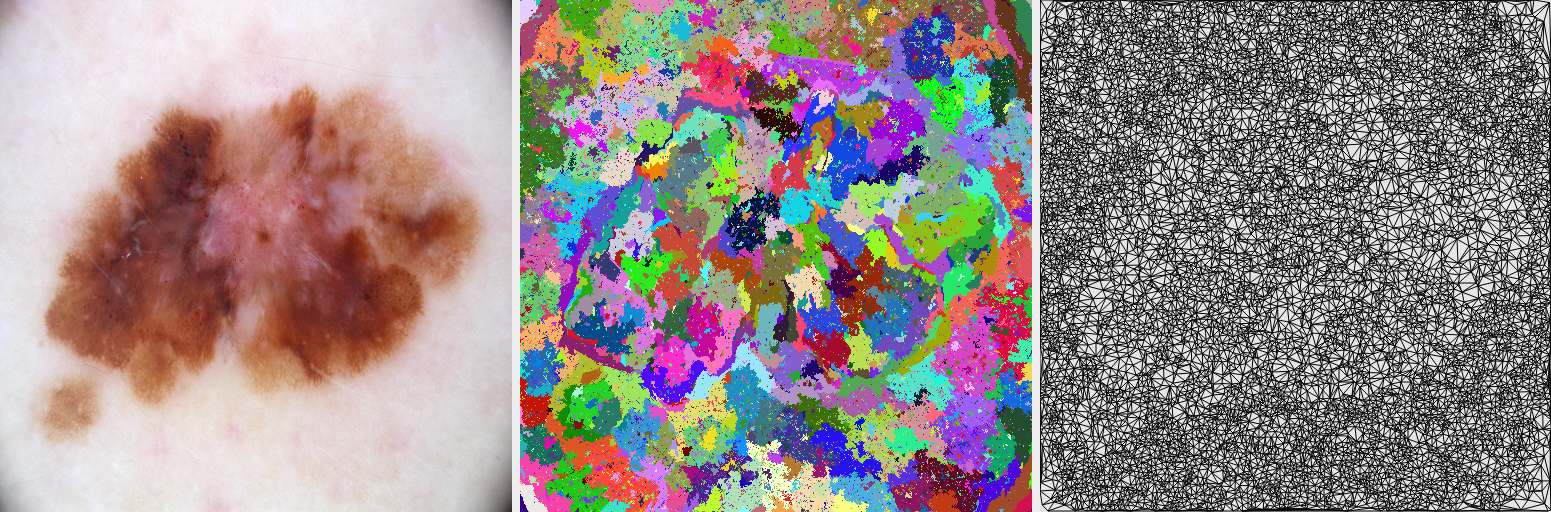
\includegraphics [width=1\textwidth] {figures/graph_ext}
			\caption{Kruskal MST based region merging \& graph extraction.}
			\label{fig:graph_extract}
		\end{center}
		\small 
		Result of applying a Kruskal based region merging algorithm to an image of numerous small scale regular structures. (1) Input image, (2) 
		
	\end{figure}


\section{Anonymity: SaNGreeA (with iML)}
\label{sect:anonymization}

	\begin{enumerate}
		\item \textbf{Process input data into suitable structure}
		\item \textbf{Enhance structure with graph information (random)}
		\item \textbf{Anonymize via SaNGreeA}
		\item \textbf{prepare individual cost function via iML}
		\item \textbf{Anonymize via SaNGreeA modified}
		\item \textbf{Compare results}
	\end{enumerate}
	
	\begin{figure}[ht]
		\label{fig_anonIML}
		\begin{center}
			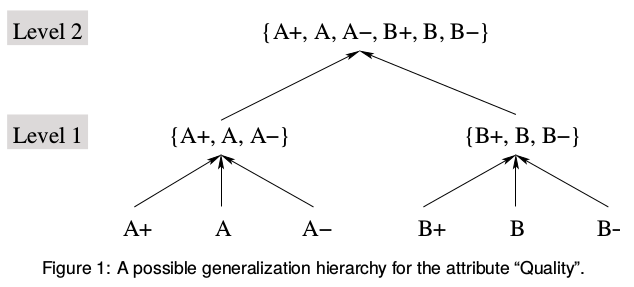
\includegraphics[width=0.8\textwidth]{figures/anonym/gen_hierarchy}
			\caption{Example of a typical generalization hierarchy}
		\end{center}
	\end{figure}	
	
	\begin{figure}[ht]
		\label{fig_anonIML}
		\begin{center}
			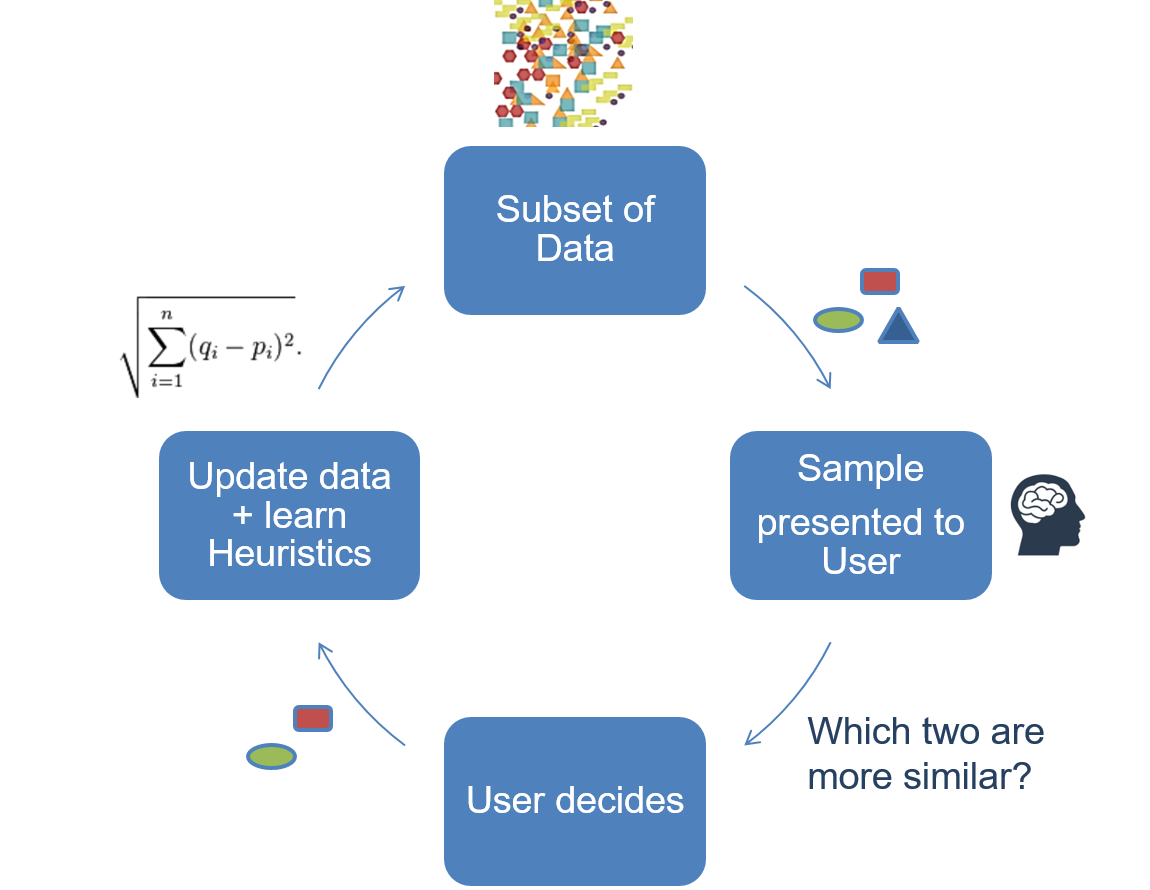
\includegraphics[width=1\textwidth]{figures/anonym/anonIML}
			\caption{Anonymization augmented by IML (human in the loop)}
		\end{center}
	\end{figure}


